\documentclass{beamer}
\usetheme{default}
\usecolortheme{seahorse}
\usepackage{graphicx}
\usepackage{epstopdf}
\usepackage[document]{ragged2e}

\title{TITLE}   
\subtitle{Experimental Economics -- oTree Project Documentation}
\author{Martin Kotek, Magdalena Rausova \& Veronika Vrana} 
\date{\today} 


\begin{document}


\frame{\titlepage} 



\begin{frame}
\frametitle{Instructions for the experiment}

\justify
In this experiment two players are matched randomly and anonymously. Each of them can decide whether to cooperate or defect. Defection leads to better outcome for the defector and worse for the other player. If both players cooperate, they can get (a,a). All combinations of outcomes are displayed in the table below.\\

To induce the cooperation of player 2, player 1 can promise a reward to player 2 in case they manage both to cooperate. Then both players decide whether to cooperate or not. If they both decide to cooperate, player 1 can decide how much to send to player 2 (independently from the original promise).\\

\begin{center}
   \begin{tabular}{lcc}
     & \textbf{cooperate} &  \textbf{defect} \\
      \textbf{cooperate} &  (a,a) & (0,b) \\
      \textbf{defect} & (b,0) & (d,d) \\    
 \end{tabular}
\end{center}

\end{frame}




\begin{frame}
\frametitle{Diagram} 

\begin{figure}[!htbp]
\begin{center}\vspace{-0.5cm}
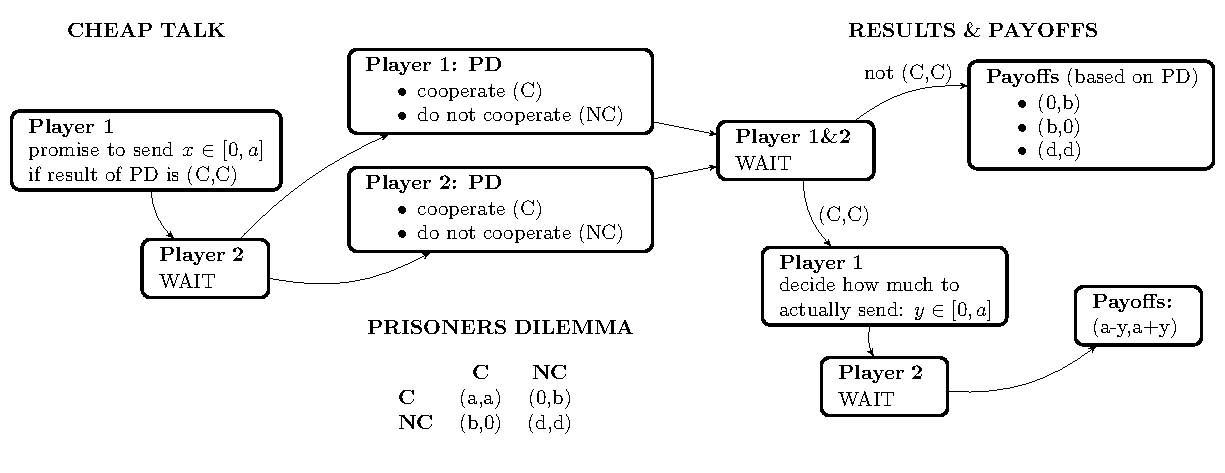
\includegraphics[width=110mm]{diagram.pdf}
\end{center}\vspace{-0.5cm}
\end{figure}

\end{frame}



 
\begin{frame}
\frametitle{models.py} 

\begin{itemize}
  \item Constants -- pay-offs in prisoner's dilemma
	\begin{itemize}
		\item $a$ -- pay-off if both players cooperate
		\item $b$ -- pay-off for non-cooperating player if the other cooperates
		\item $d$ -- pay-off if both players not cooperate
	\end{itemize}
	
  \item Player
	\begin{itemize}
	  \item Attributes for promised and actual payment
	  \item Method determining whether cooperation was successful (to determine flow of the game)
		\item Methods for calculating pay-offs based on moves
	\end{itemize}

  \item Group
	\item Subsession
\end{itemize}

\end{frame}



\begin{frame}
\frametitle{Templates} 

\begin{itemize}
  \item Submit\_cheap\_talk.html
	\begin{itemize}
		\item Screen for player 1 with form to select promised amount between 0 and $a$. 
		\item Instructions
	\end{itemize}
  
	\item Submit\_prisoner\_dilemma.html
	\begin{itemize}
		\item Standard prisoner's dilemma game for both players -- buttons to select a strategy.
		\item Instructions
	\end{itemize}
  
	\item Submit\_actual.html
	\begin{itemize}
		\item Displayed only in case of successful cooperation. Contains a form to select actual payment between 0 and $a$. 
	\end{itemize}

	\item Results.html
	\begin{itemize}
		\item Display final results of the round. 
	\end{itemize}	

\end{itemize}

\end{frame}




\begin{frame}
\frametitle{views.py} 

\begin{itemize}
  \item Submit cheap talk
	\begin{itemize}
		\item Screen for player 1 where she decides how much she promises to pay in case of successful cooperation.
	\end{itemize}
  
	\item Waiting screen
	\begin{itemize}
		\item Wait until player 1 decides how much she promises to pay in case of successful cooperation. 
	\end{itemize}
	
	\item Submit prisoner dilemma
	\begin{itemize}
		\item Standard prisoner's dilemma game for both players.
	\end{itemize}
	
	\item Waiting screen
	\begin{itemize}
		\item Wait until both players decide about their moves in prisoner's dilemma. Decide about the next screen and calculate pay-offs if game ends.
	\end{itemize}

\end{itemize}
\end{frame}


\begin{frame}
\frametitle{views.py} 

\begin{itemize}  
	\item Submit actual
	\begin{itemize}
		\item Displayed only in case of successful cooperation. Player 1 decides how much to pay to the player 2.
	\end{itemize}
	
	\item Waiting screen
	\begin{itemize}
		\item Displayed only in case of successful cooperation. Wait until player 1 decides how much she pays to the player 2. Calculate pay-offs.
	\end{itemize}
	
	\item Results
	\begin{itemize}
		\item Display final results of the round. There are two different results screens -- for successful cooperation and for other outcomes
	\end{itemize}	

\end{itemize}
\end{frame}



\end{document}

